\chapter{Результаты апробации методов на экземпляре \texttt{full\_arbiter\_3} с соревнования SYNTCOMP}%
\label{app:syntcomp}

\begin{figure}[!h]
    \centering
    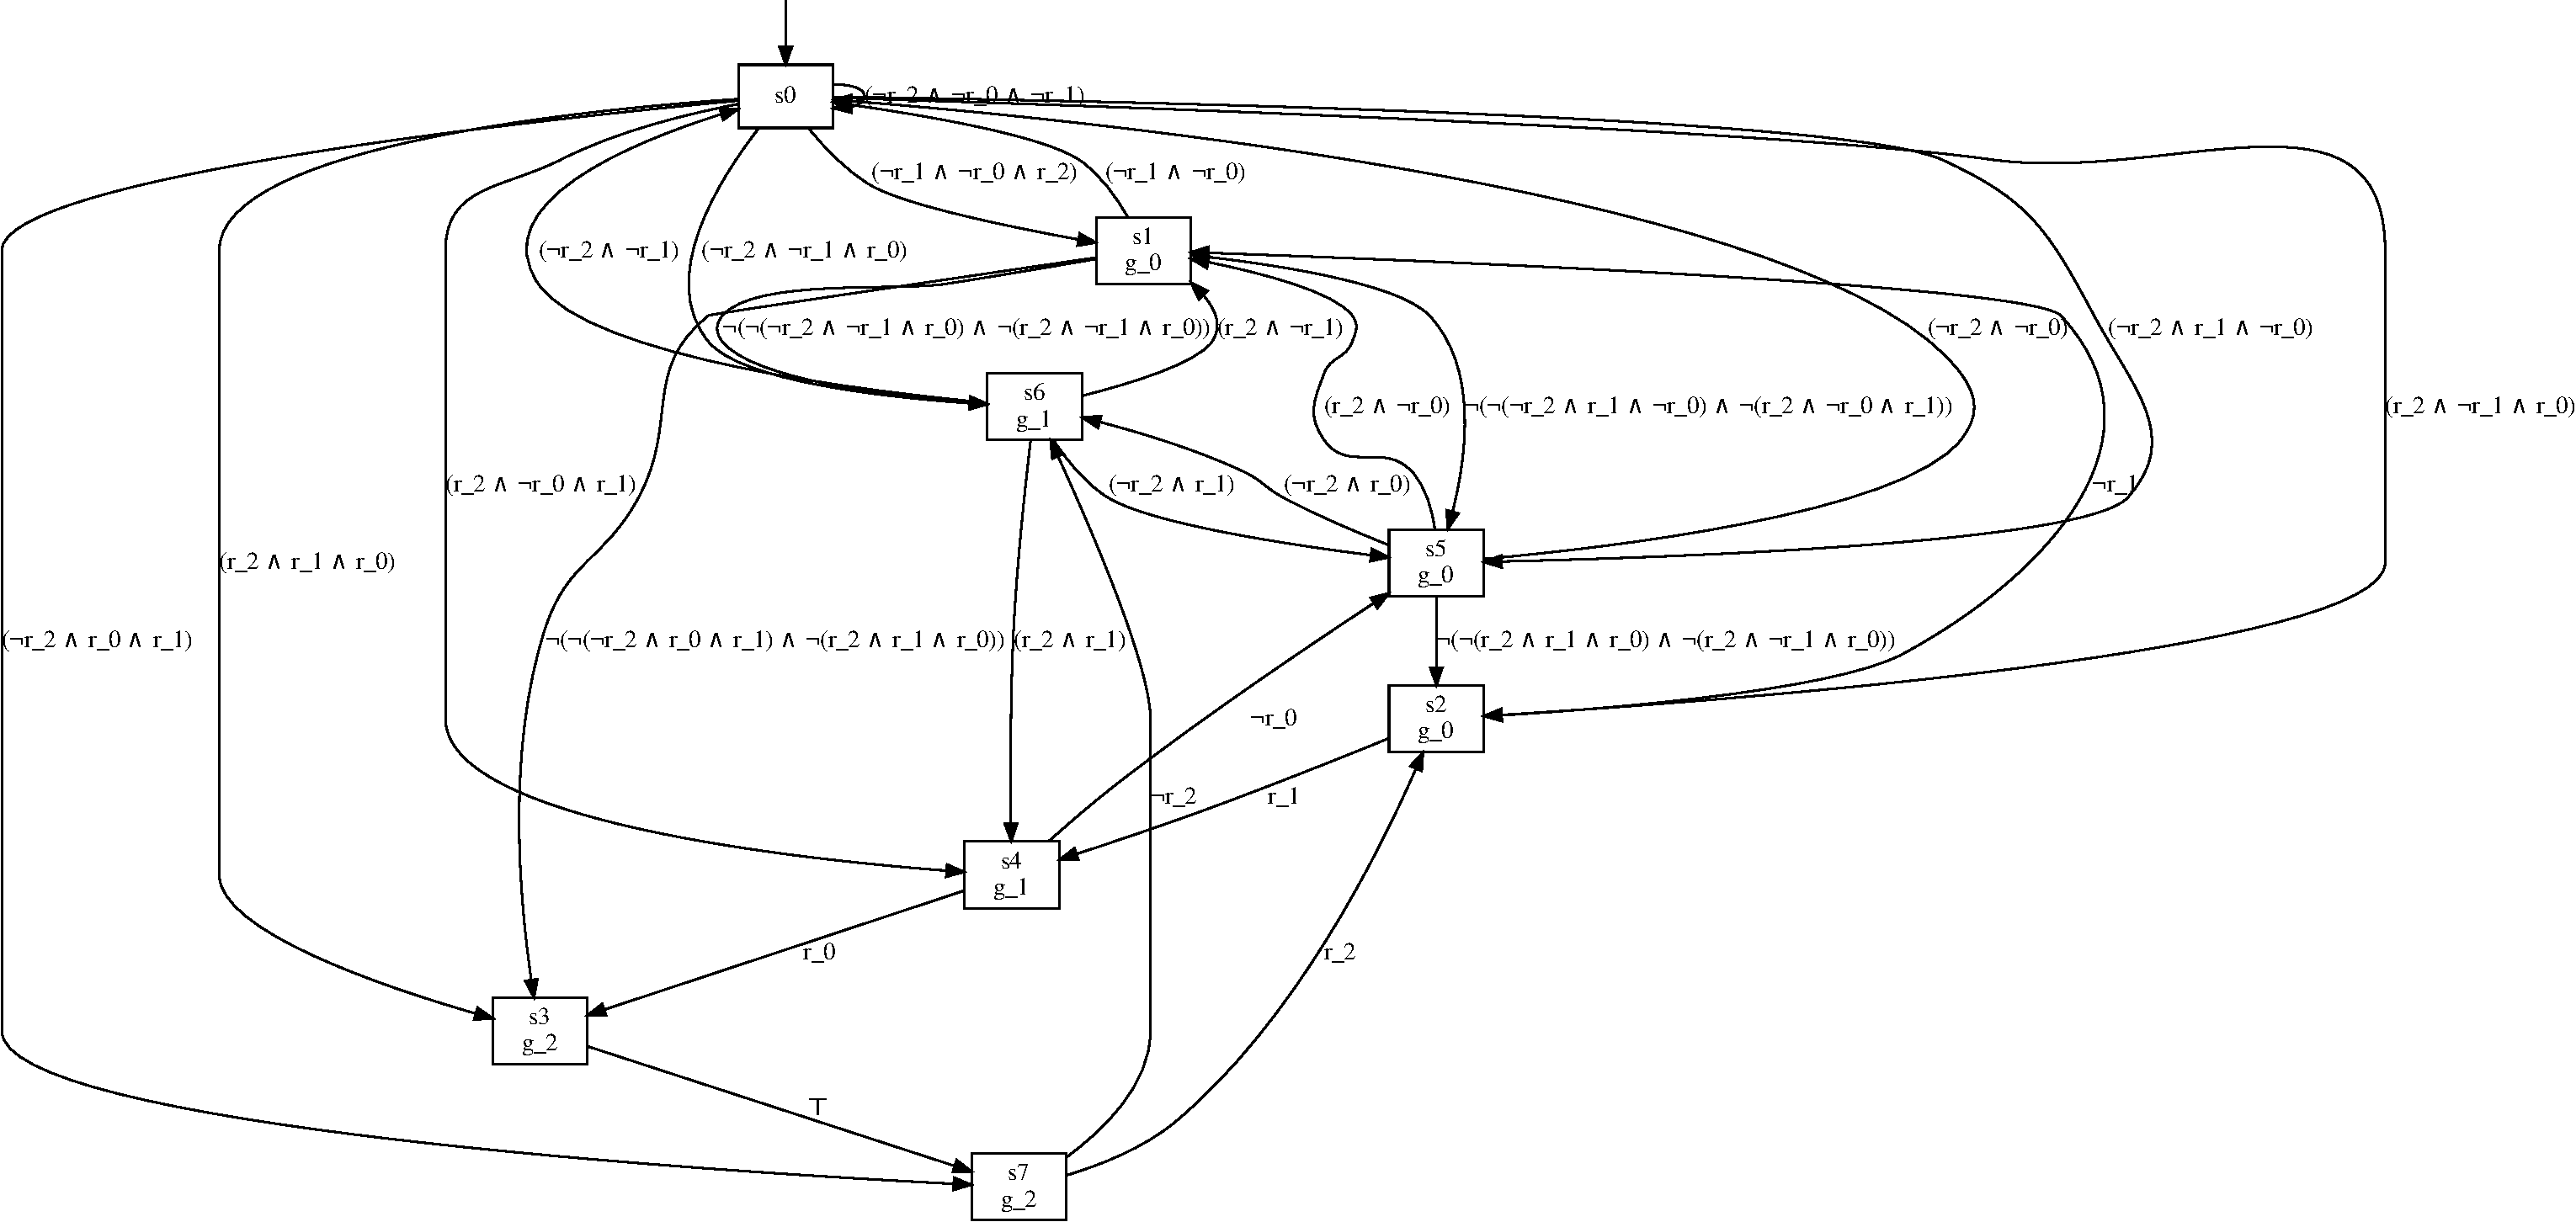
\includegraphics[rotate=90, width=\textwidth, max height=\maxheight{3}-100pt]{images/syntcomp-bosy.pdf}
    \caption{Система переходов $\mathcal{T}_{\text{original}}$, полученная с помощью BoSy для инстанса \texttt{full\_arbiter\_3}: ${C = 8}$ состояний, ${T = 28}$ переходов, суммарный размер охранных условий ${N = 147}$}%
    \label{fig:syntcomp-bosy}
\end{figure}

\begin{figure}[p]
    \centering
    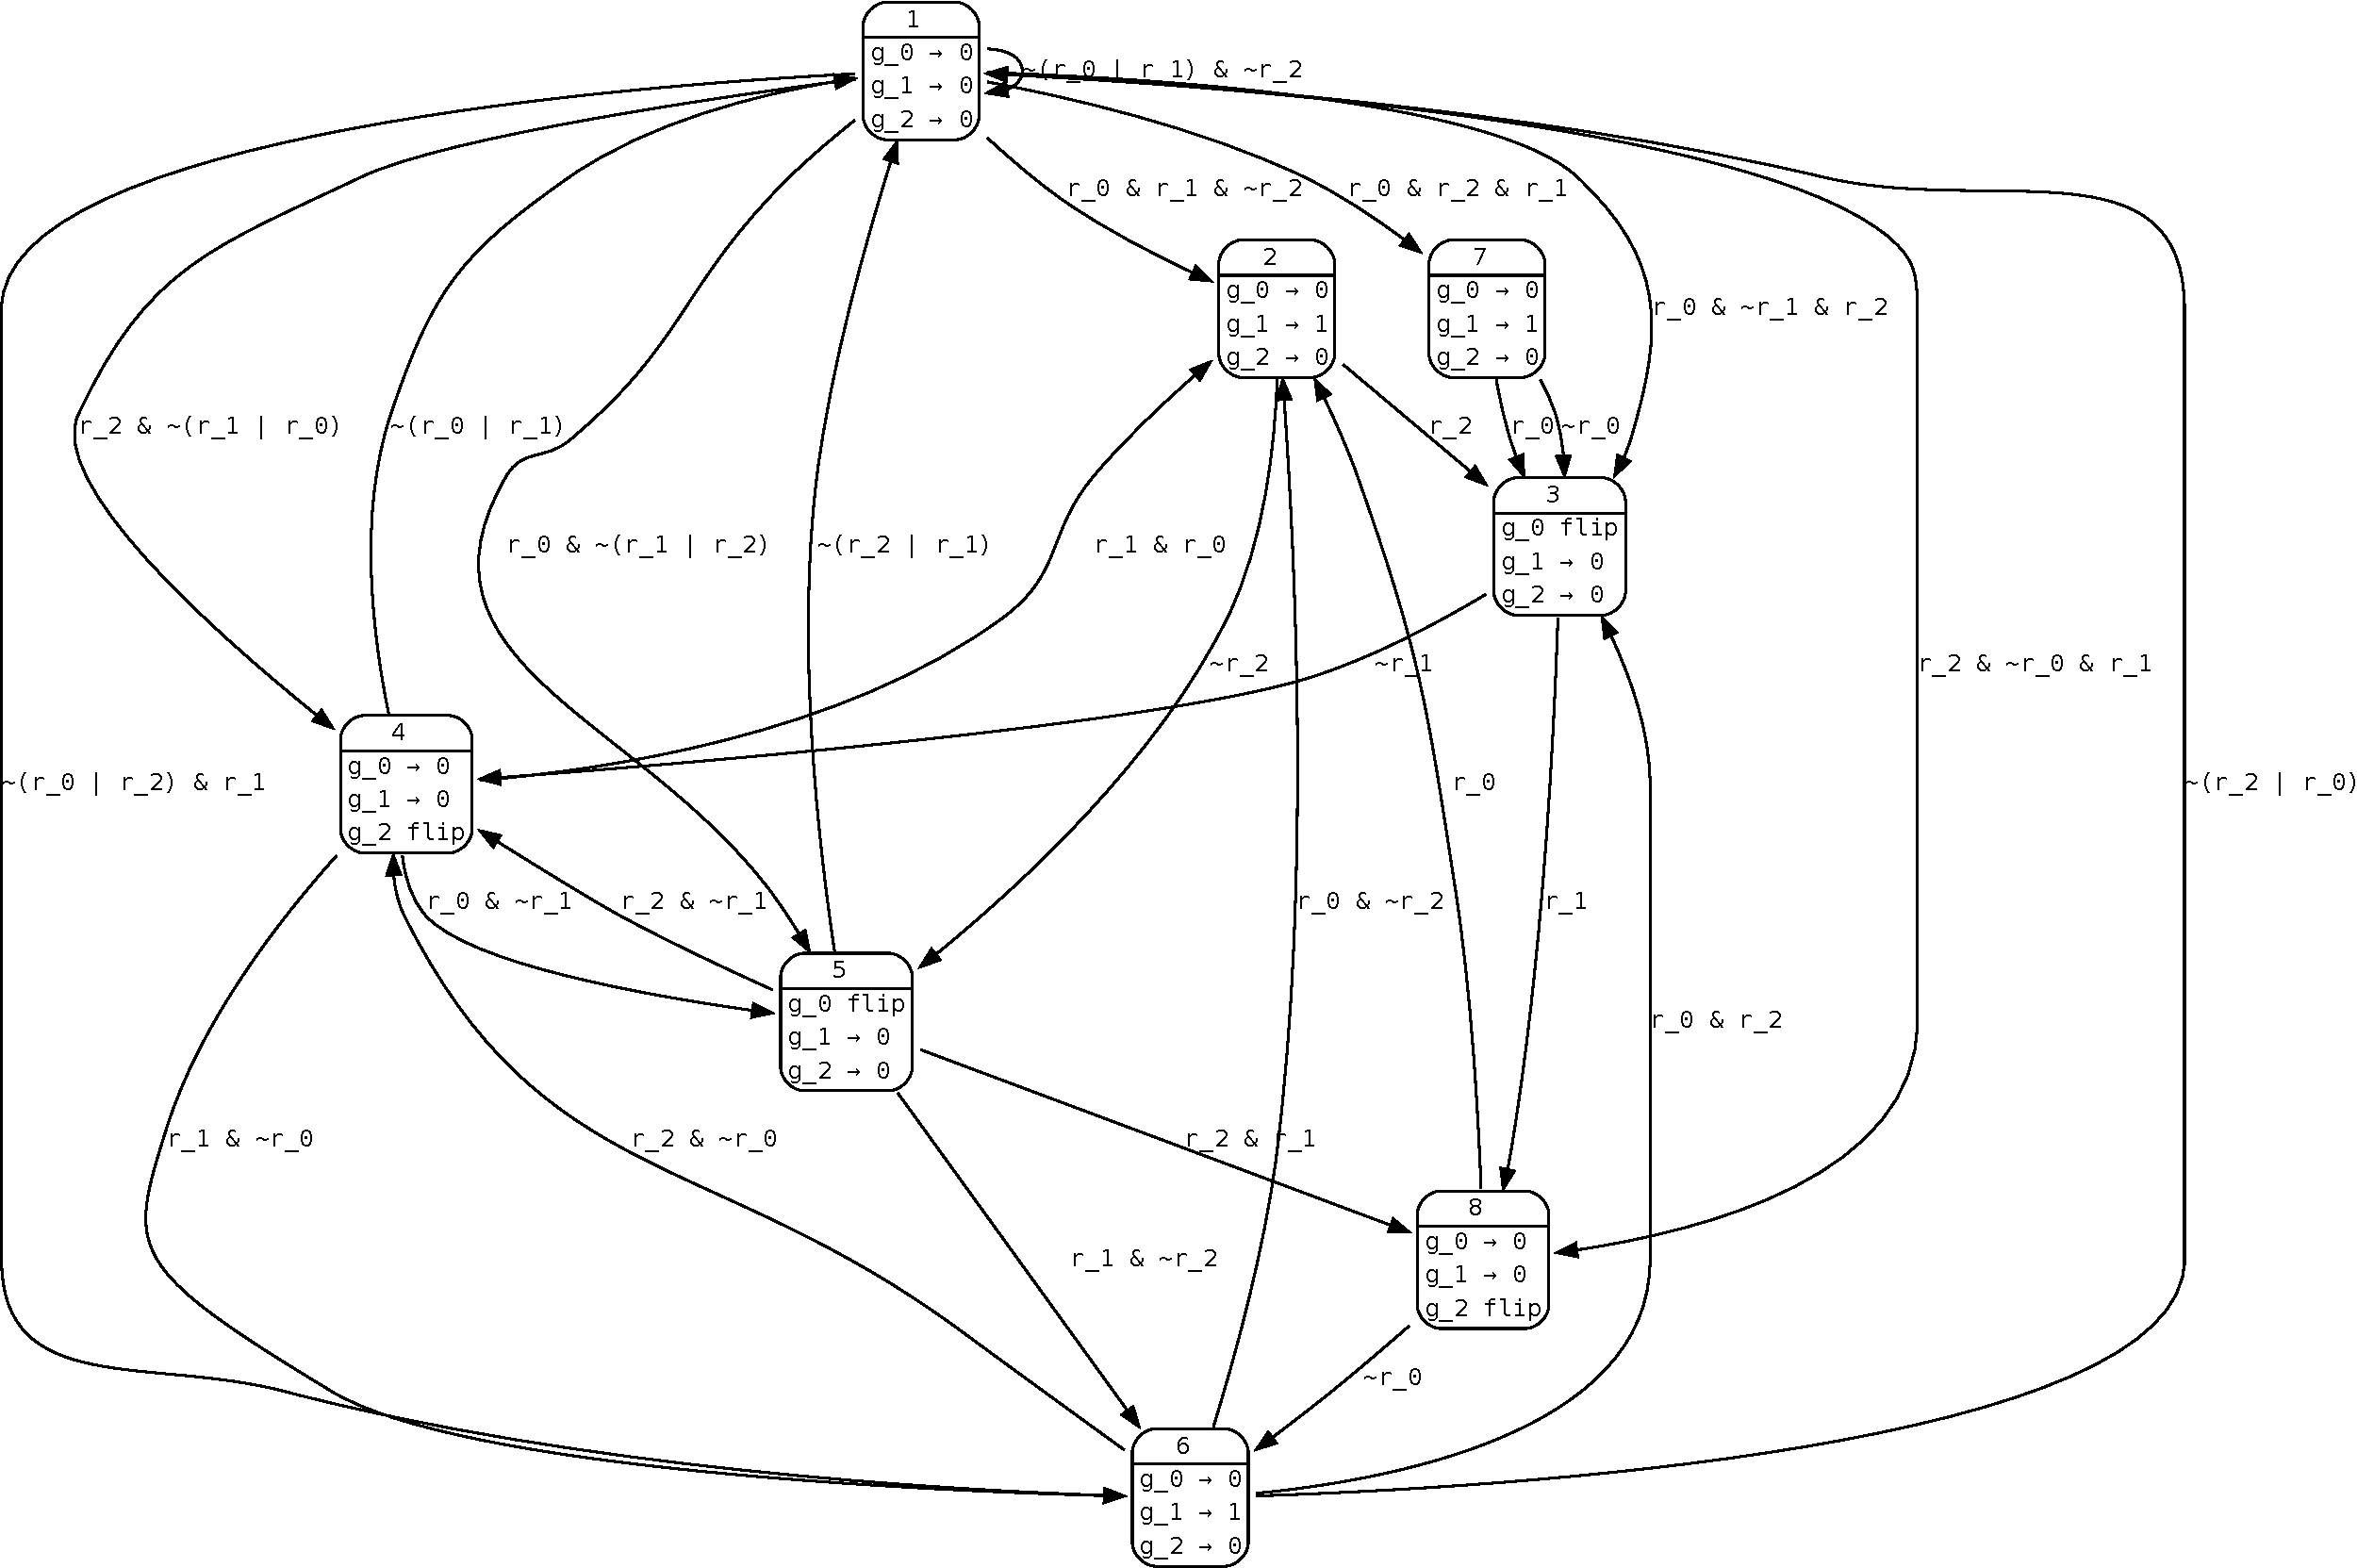
\includegraphics[rotate=90, width=\textwidth, max height=\maxheight{3}]{images/syntcomp-fbsat-deterministic.pdf}
    \caption{Детерминированная минимизированная система переходов $\Automaton_{\text{deterministic}}$, полученная с помощью \smallcaps{fbSAT}, с меньшим суммарными размером охранных условий:~${N = 105}$}%
    \label{fig:syntcomp-fbsat-deterministic}
\end{figure}

\begin{figure}[p]
    \centering
    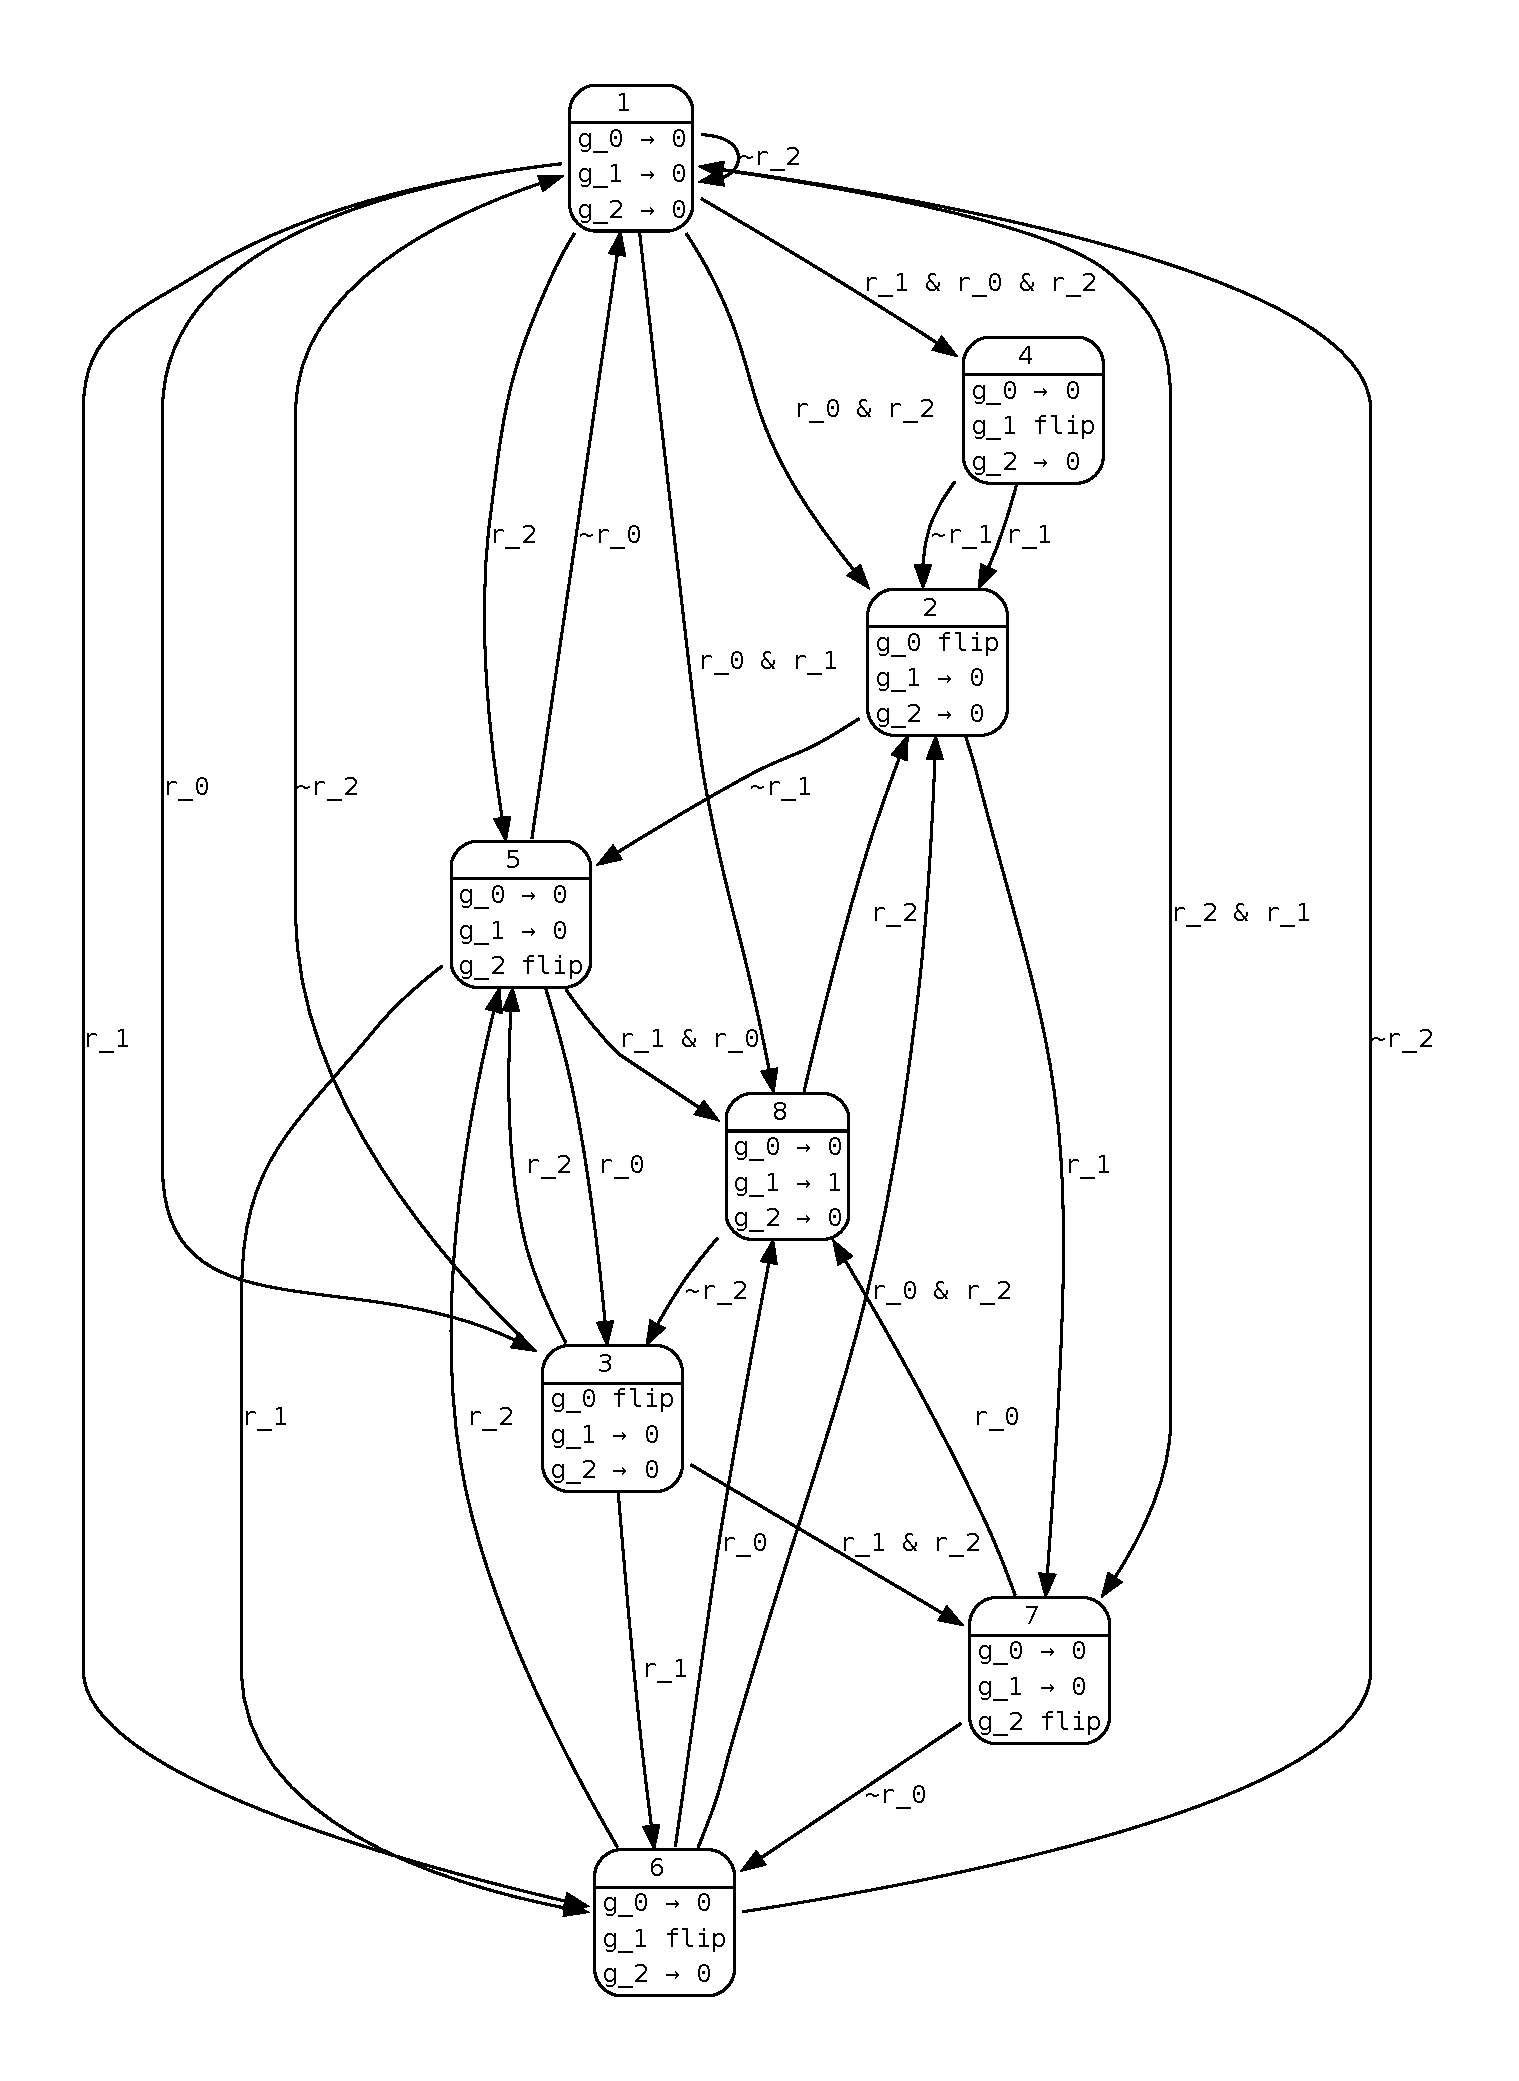
\includegraphics[width=\textwidth, max height=\maxheight{3}]{images/syntcomp-fbsat.pdf}
    \caption{Минимальная недетерминированная система переходов $\Automaton_{\text{non-deterministic}}$, полученная с помощью \smallcaps{fbSAT}, с ещё меньшим суммарным размером охранных условий:~${N = 52}$}%
    \label{fig:syntcomp-fbsat}
\end{figure}


\iffalse

\chapter{Основные публикации автора по теме диссертации}
\label{app:publications}

\newcommand{\mypublication}[2][-]{% [<pages>]{<path>}
    \includepdf[
        pages={#1},
        pagecommand={},  % to include global numbering
        scale=0.9,  % to leave space for the global page numbers
        frame, % (optional)
    ]{#2}
}

\begin{refsection}[biblio/own.bib]
\nocite{
    chivilikhin2020,%%% PLC
    chukharev2020,%%%%% CEGIS
    chukharev2020b,%%%% BF
    chukharev2022,%%%%% fbSAT
    semenov2022,%%%%%%% LEC
    andreev2024%%%%%%%% IMP
}
\printbibliography[
    keyword=own,
    % title={Список всех публикаций автора по теме диссертации},
    % heading=subbibliography,
    heading=none,
    resetnumbers=true
]
\end{refsection}

% \begin{enumerate}[beginpenalty=10000, left=0pt]
%     \item D.~Chivilikhin, S.~Patil, K.~Chukharev, A.~Cordonnier, and V.~Vyatkin, ``Automatic state machine reconstruction from legacy PLC using data collection and SAT solver'', \textit{IEEE Transactions on Industrial Informatics}, vol.~16, pp.~\np{7821}--\np{7831}, 2020.
%     \item K.~Chukharev, D.~Suvorov, D.~Chivilikhin, and V. Vyatkin, “SAT-based counterexample- guided inductive synthesis of distributed controllers”, \textit{IEEE Access}, vol.~8, pp.~\np{207485}--\np{207498}, 2020.
%     \item К.~Чухарев, <<Применение инкрементальных SAT-решателей для решения NP-трудных задач на примере задачи синтеза минимальных булевых формул>>, \textit{Научно-технический вестник информационных технологий, механики и оптики}, т.~20, №~6(130), с.~841--847, 2020.
%     \item K.~Chukharev and D.~Chivilikhin, ``fbSAT: Automatic inference of minimal finite-state
%     models of function blocks using SAT solver'', \textit{IEEE Access}, vol.~10, pp.~\np{131592}--\np{131610},
%     2022.
%     \item A.~Semenov, K.~Chukharev, E.~Tarasov, D.~Chivilikhin, and V.~Kondratiev, Estimating
%     the hardness of SAT encodings for Logical Equivalence Checking of Boolean circuits, 2022. arXiv: 2210.01484~[cs].
%     \item A.~Andreev, K.~Chukharev, S.~Kochemazov, and A.~Semenov, ``Solving influence maximization problem under deterministic linear threshold model using metaheuristic optimization'', in \textit{MIPRO~2024}, Opatija, Croatia, 2024.
% \end{enumerate}

\mypublication{biblio/MyPublications/2020_PLC.pdf}
\mypublication{biblio/MyPublications/2020_CEGIS.pdf}
\mypublication{biblio/MyPublications/2020_BF.pdf}
\mypublication{biblio/MyPublications/2022_fbSAT.pdf}
\mypublication{biblio/MyPublications/2022_LEC.pdf}
\mypublication{biblio/MyPublications/2024_IMP.pdf}

\fi
